\documentclass{article}
\usepackage{graphicx} % Required for inserting images
\usepackage{listings} % Required for insertion of code
\usepackage{amsmath} % Required for math features
\usepackage{hyperref} % Required for adding hyperlinks
\usepackage{booktabs} % Required for better table formats
\usepackage[top=1in, bottom=1in, left=1in, right=1in]{geometry} % Adjust the page margins
\usepackage{placeins} % Required to use \FloatBarrier to ensure figures are shown before section ends
\usepackage{amssymb} % Required for math symbols
\usepackage{algorithm}
\usepackage{algpseudocode}

\title{CMOR 421 Homework 2: OpenMP}
\author{Hubert King}
\date{March 25th, 2024}

\begin{document}

\maketitle

\section{Blocked Matrix-Matrix Multiplication using OpenMP}
\subsection{Instructions}
Optimize blocked matmul using OpenMP. You may run this on either your own laptop or on NOTS. Compare \texttt{\#omp parallel for} with \texttt{\#omp parallel for collapse(2)}. Report the parallel efficiency as you increase the number of threads.
\subsection{Solution}

Timing data and parallel efficiency for serial and parallel implementations of blocked matrix-matrix multiplication using  \texttt{\#omp parallel for} with \texttt{\#omp parallel for collapse(2)} are summarized below. As the number of threads increased, the parallel efficiency decreased, likely due to the overhead incurred from spawning new threads. The collapse directive improved efficiency, likely due to more efficient work load balancing as the number of threads increased. Since the outer loop's size is determined by the block size, there were more threads than iterations when $threads > 8$. This is where the difference in efficiencies is greatest; the collapse directive ensures that the number of iterations in the loop is greater than the threads available.
\begin{table}[h!]
\centering
\begin{tabular}{@{}lccccc@{}}
\toprule
Number of Threads & 8 & 12 & 16 & 20 & 24 \\
\midrule
Serial (s) & 2.51 & 2.51 & 2.51 & 2.52 & 2.51 \\
Nested Parallel (s) & 0.323 & 0.338 & 0.337 & 0.360 & 0.363 \\
Collapse Parallel (s) & 0.305 & 0.233 & 0.232 & 0.262 & 0.319 \\
\bottomrule
\end{tabular}
\caption{Blocked matrix multiplication execution time for serial and parallel implementations using nested parallelism and collapse directive. Timings reflect the total execution time for five trials. For all trials, block size was $n = 8$}
\label{tab:matmul_times}
\end{table}

\FloatBarrier

\begin{figure}
    \centering
    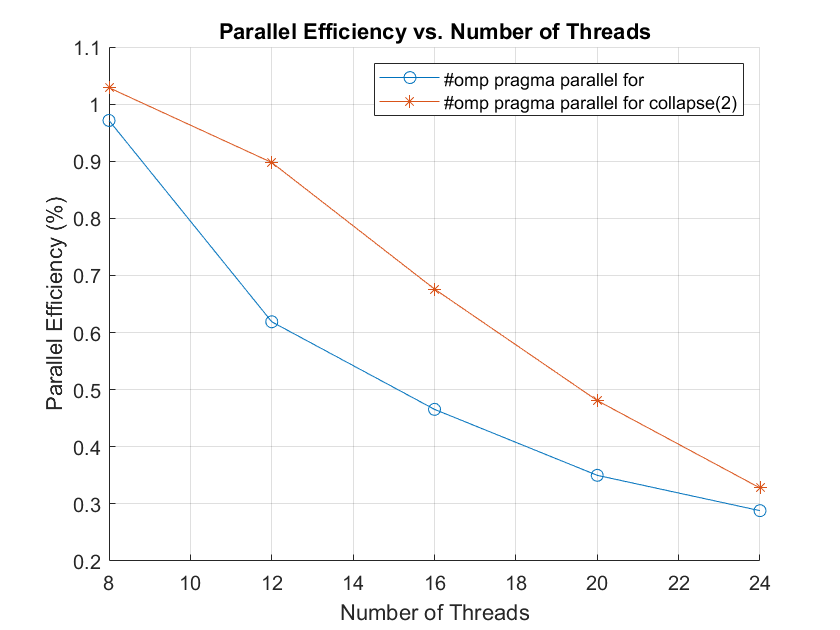
\includegraphics[height=10cm]{part_1_parr_eff.png}
    \caption{Parallel efficiency plot for parallel back solve algorithm with static scheduling. Five trials were run and eight threads were used.}
    \label{fig:enter-label}
\end{figure}
\FloatBarrier

\section{Parallel Back Solve with Unit Upper Triangular Matrix}
\subsection{Intructions}
Parallel back solve with a unit upper triangular matrix. Write out the back solve algorithm explicitly and identify parallelism. Provide pseudocode, and implement your algorithm in C++ using OpenMP. For a sufficiently large matrix size, test your implementation: Does static or dynamic scheduling work better? Why? Test your implementation for several matrix sizes and report the parallel efficiency as a function of matrix size. Do you expect parallel efficiency to be better or worse if the lower triangular matrix is only bi-diagonal?


\subsection{Solution}
Given a system $Ax = b$, where $A$ is an $n \times n$ unit upper triangular matrix with any upper entries, and $b$ is the right-hand side vector, the matrix $A$ and vector $b$ can be represented as:

\[
A = \begin{bmatrix}
1 & a_{12} & a_{13} & \cdots & a_{1n} \\
0 & 1 & a_{23} & \cdots & a_{2n} \\
0 & 0 & 1 & \ddots & \vdots \\
\vdots & \vdots & \ddots & \ddots & a_{(n-1)n} \\
0 & 0 & \cdots & 0 & 1 \\
\end{bmatrix}, 
\quad b = \begin{bmatrix}
b_{1} \\
b_{2} \\
\vdots \\
b_{n} \\
\end{bmatrix}
\]

The equations derived from this system are for $i = 1, \ldots, n$:

\[
x_i + \sum_{j=i+1}^{n} a_{ij}x_j = b_i
\]

This system can be solved using the back solve algorithm below. This approach iterates through rows in the outer loop and columns in the inner loop.

\begin{algorithm}
\caption{Back Solve with Unit Upper Triangular Matrix}
\begin{algorithmic}
\State \textbf{Input:} $A$ (an $n \times n$ unit upper triangular matrix), $b$ (vector in $\mathbb{R}^n$), n (dimension of A)
\State \textbf{Output:} $x$ (vector in $\mathbb{R}^n$)
\For{$i = 1,...,n$}
    \State $x_i = b_i$
\EndFor
\For{$j = n,...,1$}
    \For{$i = 1,...,j$}
        \State Compute $x_i = x_i - A_{ij} \cdot x_j$
    \EndFor
\EndFor
\State \textbf{return} $x$
\end{algorithmic}
\end{algorithm}
\FloatBarrier 
Algorithm 2 uses a parallel for-loop to assign values of $b$ to $x$, and another parallel for-loop to adjust x as the inner loop of the nested for-loop iterates through rows of $A$.
\begin{algorithm}
\caption{Back Solve with Unit Upper Triangular Matrix}
\begin{algorithmic}
\State \textbf{Input:} $A$ (an $n \times n$ unit upper triangular matrix), $b$ (vector in $\mathbb{R}^n$), n (dimension of A)
\State \textbf{Output:} $x$ (vector in $\mathbb{R}^n$)
\State \textbf{Parallel for-loop}: distribute for-loop across threads
\For{$i = 1,...,n$}
    \State $x_i = b_i$
\EndFor
\For{$j = n,...,1$}
    \State \textbf{Parallel for-loop}: distribute for-loop across threads
    \For{$i = 1,...,j$}
        \State Compute $x_i = x_i - A_{ij} \cdot x_j$
    \EndFor
\EndFor
\State \textbf{return} $x$
\end{algorithmic}
\end{algorithm}
\FloatBarrier
Timing Data and parallel efficiency are summarized below. Each algorithm was run for five trials, with eight threads. The effects of parrallelization were observed with $n > 3000$. Static scheduling had better effects on execution time than dynamic scheduling. This could be explained by the extra overhead incurred by dynamic scheduling. While operations per iteration in the inner for-loop do vary, meaning dynamic scheduling should improve performance, the benefit may not be enough to offset the extra overhead experienced. 

For a bi-diagonal unit upper triangular matrix, parallel efficiency would likely be greater, since the inner loop performs exactly two operations per loop. Thus, the spread of work across threads is maximally efficient with the least possible downtime. Thus, static scheduling could be used with no risk of load imbalance. If we consider the grocery checkout analogy presented in class, this means that all cashiers have two customers at a time, and would get new customers simultaneously with no downtime.

\begin{table}[h!]
\centering
\begin{tabular}{@{}lcccccccccc@{}}
\toprule
Matrix Size & 3000 & 6000 & 9000 & 12000 & 15000 & 18000 & 21000 & 24000 & 27000 & 30000 \\
\midrule
Serial (s) & 0.130 & 0.662 & 1.49 & 2.82 & 4.29 & 6.30 & 9.73 & 17.28 & 14.5 & 18.3 \\
Static (s) & 0.114 & 0.236 & 0.414 & 0.87 & 0.98 & 1.43 & 2.29 & 3.42 & 2.65 & 3.37 \\
Dynamic (s) & 1.93 & 8.39 & 18.3 & - & - & - & - & - & - & - \\
\bottomrule
\end{tabular}
\caption{Back Solve algorithm execution time for serial implementation and parallel implementation with static and dynamic scheduling. All implementations used eight threads. Dynamic timings were omitted past $n = 9000$, and values reflect the total execution time for five trials.}
\label{tab:back_solve_times}
\end{table}


\FloatBarrier
\begin{figure}
    \centering
    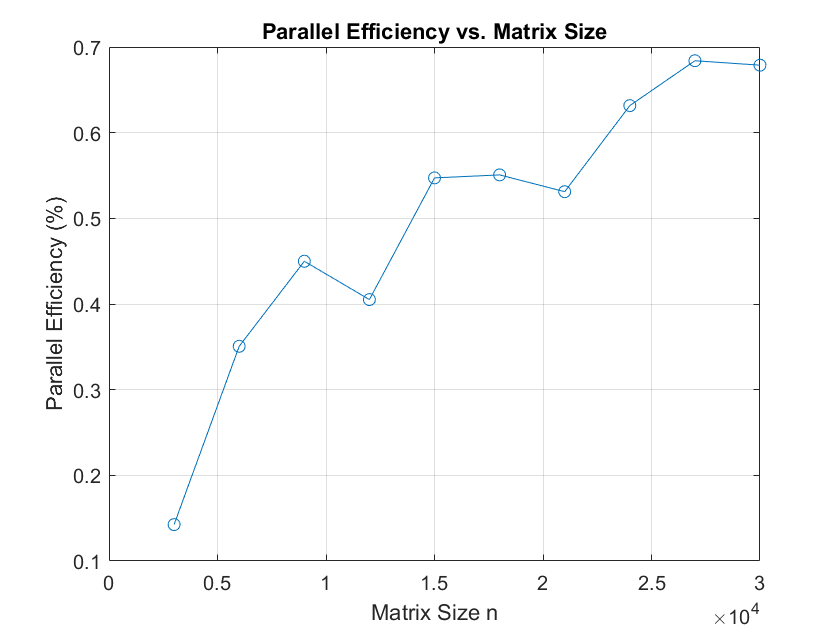
\includegraphics[height=10cm]{part_2_parr_eff.png}
    \caption{Parallel efficiency plot for parallel back solve algorithm with static scheduling. Five trials were run and eight threads were used.}
    \label{fig:enter-label}
\end{figure}
\FloatBarrier

\section{Build and Run Instructions}
\subsection{Prerequisites}
Ensure the following requirements are met:
\begin{itemize}
    \item The instructions are intended for users on the NOTS system.
    \item GCC version 13.1.0 is necessary for successful compilation and execution of the rmatmul.cpp.
\end{itemize}
\subsection{Build and Run}
Access NOTS via a login node and load the necessary modules:
\begin{verbatim}
module load GCCcore/13.1.0
\end{verbatim}
Verify that the module is loaded correctly and the correct version of GCC is being used:
\begin{verbatim}gcc --version\end{verbatim}
Next, compile the program with the following command:
\begin{verbatim}
g++ -fopenmp -o main -Iinclude main.cpp src/functions.cpp
\end{verbatim}
After successful compilation, the program can be tested by running the following command in the interactive node, where dimension is replaced by the desired matrix size. This size will be used for both blocked matrix-matrix multiplication and back-solve algorithms.
\begin{verbatim}
./main <dimension>
\end{verbatim}
To see the effects of multi-threading, access an interactive node and specify that 24 CPUs are to be allocated:
\begin{verbatim}
srun --partition=interactive --pty --export=ALL --cpus-per-task=24 --time=00:30:00 /bin/bash
\end{verbatim}
Now, run the executable as before:
\begin{verbatim}
./main <dimension>
\end{verbatim}
\end{document}
